% ==============================================================================
% ================================= Aufgabe 4 =================================
% ==============================================================================

\chapter{Aufgabe 4: Validierung und Umfrageformular}
\label{chap:aufgabe4}
\thispagestyle{fancy}

In dieser Aufgabe wird die Logik zur Validierung des Teilnehmernamens implementiert und das Umfrageformular mit den fünf Fragen erstellt.

\section{Logik der Namensvalidierung}

Die Datei \texttt{survey.php} wird um folgende Funktionalität erweitert:

\begin{enumerate}
    \item Der übergebene Name wird aus dem GET-Parameter ausgelesen.
    \item Es wird geprüft, ob der Name bereits in der Tabelle \texttt{user\_table} existiert.
    \item Falls ja: Ausgabe einer Fehlermeldung und Abbruch.
    \item Falls der Name leer ist: Verwendung von \texttt{anonymous}.
    \item Falls \texttt{anonymous} bereits existiert, wird kein neuer Datensatz angelegt.
    \item Bei einem neuen Namen wird ein neuer Datensatz in \texttt{user\_table} angelegt.
    \item Nach erfolgreicher Validierung wird das Umfrageformular angezeigt.
\end{enumerate}

\subsection{Code der Validierung}

Die zentrale Validierungslogik in \texttt{survey.php}:

\lstinputlisting[
    language=php,
    caption={Validierungslogik in \texttt{survey.php}},
    label={lst:validation-logic}
]{asset/code/Aufgabe4.tex}

\subsection{Fehlerbehandlung}

Bei einem bereits existierenden Nutzer wird folgende Meldung angezeigt:

\begin{figure}[H]
    \centering
    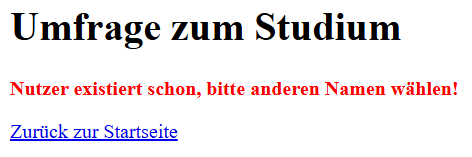
\includegraphics[width=0.5\textwidth]{./asset/image/Aufgabe4.png}
    \caption[Fehlermeldung: existierender Nutzer (\textit{Quelle: Eigene Darstellung})]
            {Fehlermeldung: existierender Nutzer (\textit{Quelle: Eigene Darstellung})\\ 
            \url{http://localhost/survey/survey.php?name=Tomakin}}
    \label{fig:error}
\end{figure}

\section{Umfrageformular}

Nach erfolgreicher Validierung wird das Umfrageformular mit fünf Fragen angezeigt:

\begin{figure}[H]
    \centering
    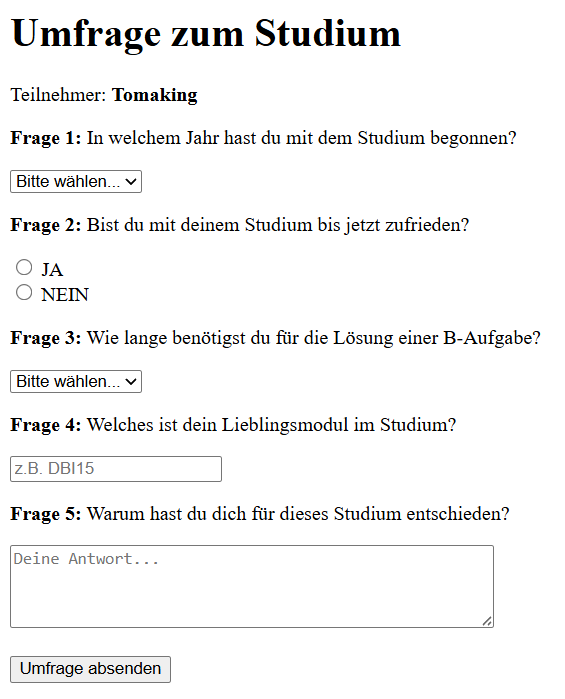
\includegraphics[width=0.7\textwidth]{./asset/image/Aufgabe4II.png}
    \caption[Umfrageformular mit fünf Fragen (\textit{Quelle: Eigene Darstellung})]
            {Umfrageformular mit fünf Fragen (\textit{Quelle: Eigene Darstellung})\\ 
            \url{http://localhost/survey/survey.php?name=Tomakin}}
    \label{fig:survey_form}
\end{figure}

\subsection{Die fünf Fragen}

\begin{table}[h]
\centering
\begin{tabular}{|c|l|l|}
\hline
\textbf{Frage} & \textbf{Inhalt} & \textbf{Eingabetyp} \\
\hline
1 & In welchem Jahr hast du mit dem Studium begonnen? & Select (\textit{Dropdown}) \\
2 & Bist du mit deinem Studium bis jetzt zufrieden? & Radio (\textit{JA/NEIN}) \\
3 & Wie lange benötigst du für die Lösung einer B-Aufgabe? & Select (\textit{Dropdown}) \\
4 & Welches ist dein Lieblingsmodul im Studium? & Textfeld \\
5 & Warum hast du dich für dieses Studium entschieden? & Textarea \\
\hline
\end{tabular}
\caption{Übersicht der fünf Umfragefragen}
\label{tab:questions}
\end{table}

\subsection{Der Quellcode des Formulars der \texttt{survey.php}}

\lstinputlisting[
    language=php,
    caption={Vollständige \texttt{survey.php} mit Validierung und Formular},
    label={lst:survey-full}
]{asset/code/Aufgabe4II.tex}

\section{Zusammenfassung}

Die Validierungslogik wurde erfolgreich implementiert:

\begin{itemize}
    \item Existierende Nutzer werden erkannt und erhalten eine Fehlermeldung.
    \item Leere Eingaben werden als \texttt{anonymous} behandelt.
    \item \texttt{anonymous} wird nur einmal in der Datenbank angelegt.
    \item Neue Nutzer werden automatisch in \texttt{user\_table} registriert.
    \item Das Umfrageformular wird mit fünf Fragen in verschiedenen Eingabetypen angezeigt.
    \item Die Nutzer-ID wird im Hidden-Feld für die weitere Verarbeitung in \texttt{save.php} bereitgehalten.
\end{itemize}

Die Datei \texttt{survey.php} liegt unter folgendem Pfad:

\begin{forest}
    for tree={
        font=\ttfamily,
        grow'=0,
        child anchor=west,
        parent anchor=south,
        anchor=west,
        calign=first,
        edge path={
            \noexpand\path [draw, \forestoption{edge}] (!u.south west) +(10pt,0) |- node[fill,inner sep=1.5pt] {} (.child anchor)\forestoption{edge label};
        },
        before typesetting nodes={
            if n=1{
                insert before={[,phantom,calign with current]}
            }{}
        },
        fit=band,
        before computing xy={l=22pt},
    }
    [\textbf{C:\textbackslash xampp\textbackslash htdocs\textbackslash survey}
        [\textbf{survey.php}]
    ]
\end{forest}

Die Anwendung ist nun bereit für die Speicherung der Umfragedaten.

% ==============================================================================
% =================================== Aufgabe 4 ================================
% ==============================================================================